\chapter*{Revisión sistemática de la literatura}
\addcontentsline{toc}{chapter}{Revisión sistemática de la literatura}\label{cap:revisionLiteratura}

\section*{1. Construcción de la bitácora}
\addcontentsline{toc}{section}{Construcción de la bitácora}\label{sec:bitacora}

En búsqueda de una base teórica para la elección de una tecnología de virtualización basada en contenedores, 
se realizó una revisión del estado del arte. Esta revisión se completó en diferentes etapas:

\subsection*{1.1 Planeación}
\addcontentsline{toc}{subsection}{Planeación}\label{subsec:planeacion}

Esta etapa consistió en establecer el propósito general que se buscaba alcanzar con el SMS (\textit{Systematic Mapping Study}). 
A su vez, definió aspectos como objetivos, preguntas de investigación y métricas. Para ello, se siguió el modelo 
Objetivo-Pregunta-Métrica (\textit{Goal-Question-Metric}, GQM). A continuación, se definen los objetivos del SMS aplicado 
a las tecnologías de virtualización basadas en contenedores.

\subsubsection*{1.1.1 Definición de metas para el SMS}
\addcontentsline{toc}{subsubsection}{Definición de metas para el SMS}\label{subsubsec:metasSMS}

\begin{table}[H]
    \centering
    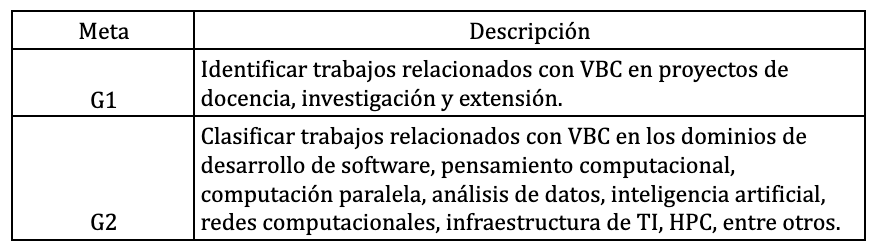
\includegraphics[width=\textwidth] {tablas-images/cp2/definicionMetas.png}
    \caption{Definición de metas del SMS}\label{tab:tabla-metas}
\end{table}

\subsubsection*{1.1.2 Definición de preguntas de investigación}
\addcontentsline{toc}{subsubsection}{Definición de preguntas de investigación}\label{subsubsec:preguntasInvestigacion}

\begin{table}[H]
    \centering
    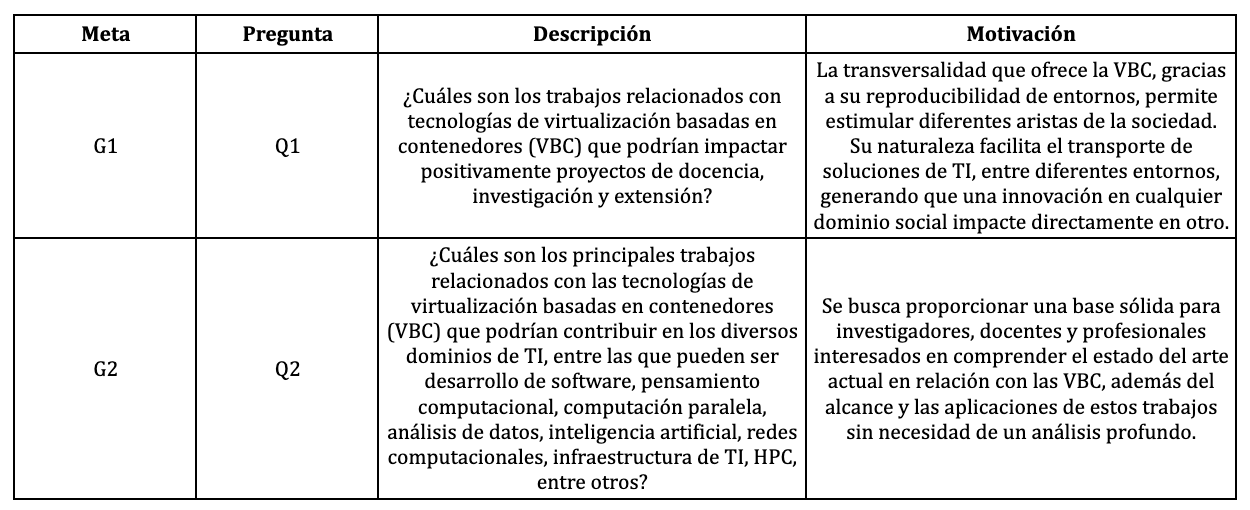
\includegraphics[width=\textwidth] {tablas-images/cp2/preguntasInvestigacion.png}
    \caption{Definición de preguntas de investigación del SMS}\label{tab:tabla-preguntas}
\end{table}

\subsubsection*{1.1.3 Definición de métricas}
\addcontentsline{toc}{subsubsection}{Definición de métricas}\label{subsubsec:metricasSMS}

\begin{figure}[H]
    \centering
    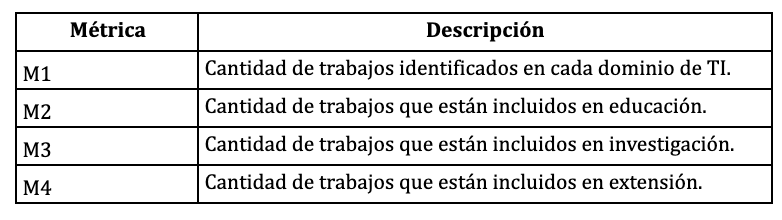
\includegraphics[width=\textwidth] {tablas-images/cp2/definicionMetricas.png}
    \caption{Definición de métricas del SMS}\label{fig:tabla-metricas}
\end{figure}

\section*{2. Búsqueda de estudios}
\addcontentsline{toc}{section}{Búsqueda de estudios}\label{sec:busquedaEstudios}

Esta etapa comprendió las siguientes secciones: 
\begin{enumerate}
  \item Estrategia de búsqueda, ya sea independiente o combinada;
  \item Identificación general de estudios;
  \item Selección; y finalmente,
  \item Selección de estudios para incluir en el SMS.
\end{enumerate}

\subsection*{2.1 Estrategia de búsqueda}
\addcontentsline{toc}{subsection}{Estrategia de búsqueda}\label{subsec:estrategiaBusqueda}

Este trabajo combinó las estrategias de búsqueda en bases de datos y búsqueda en bola de nieve. 
Para la estrategia de búsqueda en bases de datos, se seleccionaron las siguientes bases de datos: ACM, IEEE Xplore, Springer, Taylor \& Francis y Science Direct.

\subsection*{2.2 Búsqueda en bases de datos}
\addcontentsline{toc}{subsection}{Búsqueda en bases de datos}\label{subsec:busquedaBasesDatos}
Se seleccionaron las siguientes bases de datos para este propósito: ACM, IEEE Xplore, Springer, Taylor \& Francis y Science Direct.

\subsubsection*{2.2.1 Identificación de estudios mediante búsqueda en bases de datos}
\addcontentsline{toc}{subsubsection}{Identificación de estudios mediante búsqueda en bases de datos}\label{subsubsec:identificacionEstudios}
En esta etapa del proceso fue necesario establecer las palabras clave que serían útiles en las cadenas de búsqueda para cada una de las bases de datos seleccionadas. 
Los términos consideran los elementos identificados en la etapa de planificación, para lo cual también se utilizó el modelo PICOC como guía metodológica.

\begin{table}[H]
    \centering
    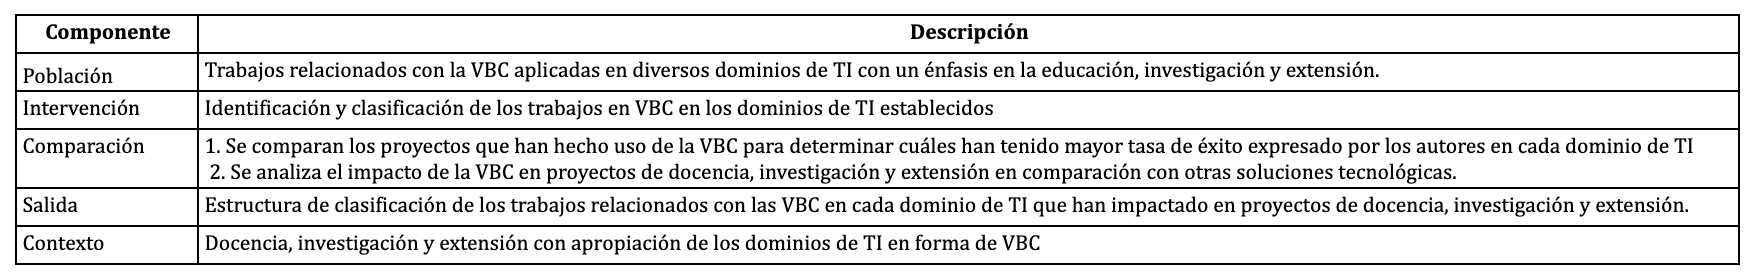
\includegraphics[width=\textwidth] {tablas-images/cp2/modelo-PICOC.png}
    \caption{Modelo PICOC}\label{tab:tabla-PICOC}
\end{table}
\begin{table}[H]
    \centering
    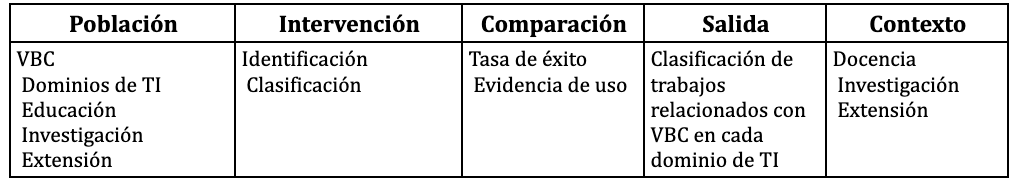
\includegraphics[width=\textwidth] {tablas-images/cp2/keywords-PICOC.png}
    \caption{Palabras clave identificadas usando el modelo PICOC}\label{tab:tabla-keywords-PICOC}
\end{table}
\begin{table}[H]
    \centering
    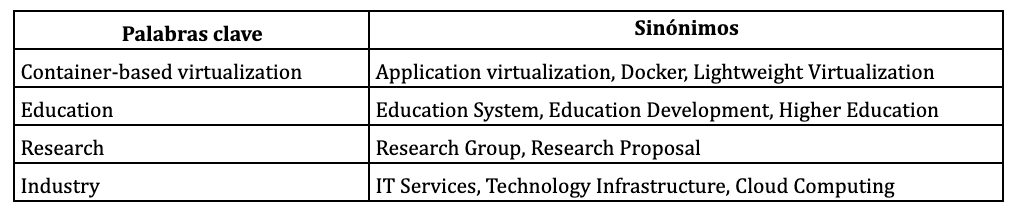
\includegraphics[width=\textwidth] {tablas-images/cp2/keywords.png}
    \caption{Palabras clave para la búsqueda en base de datos}\label{tab:tabla-keywords}
\end{table}
\begin{table}[H]
    \centering
    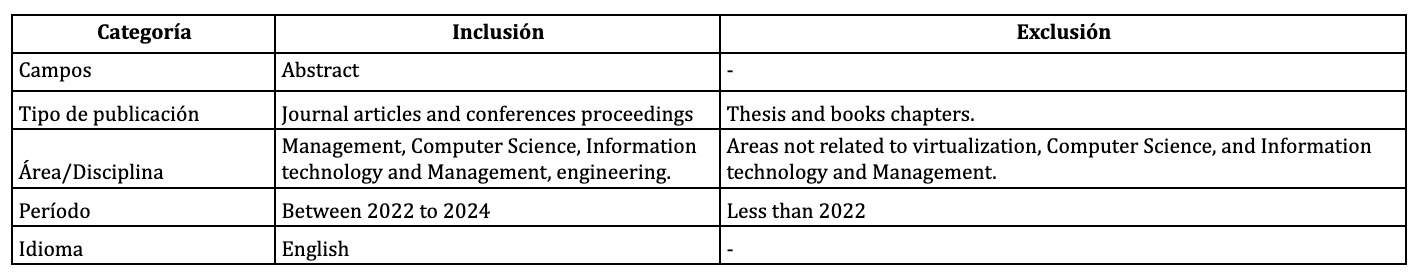
\includegraphics[width=\textwidth] {tablas-images/cp2/criterios.png}
    \caption{Criterios de Inclusión/Exclusión}\label{tab:tabla-criterios}
\end{table}

\paragraph*{2.2.1.1 Búsqueda en bases de datos}
\addcontentsline{toc}{paragraph}{2.2.1.1 Búsqueda en bases de datos}\label{par:busquedaBasesDatos}

